\newpage
\section{Agile Softwareentwicklung}
\subsection{Grundlagen}
\subsubsection{Agilität}
Definieren lässt sich Agilität unter anderem als eine Fähigkeit, sowohl Veränderungen zu schaffen als auch auf diese zu reagieren, um in einem turbulenten Geschäftsumfeld profitieren zu können. Agile Unternehmen zielen auf Veränderungen ab anstatt sie zu fürchten, da sie in der Lage sind, besser darauf zu reagieren als der Wettbewerb. Zugleich kreieren sie selbst Veränderungen, auf die Wettbewerber nur schwer antworten können und schaffen sich somit einen Vorteil. Unternehmen müssen allerdings den gewünschten Grad der Agilität bestimmen, da der dadurch erwirtschaftete Vorteil nur relativ zu den Wettbewerbern gesehen werden kann.\footcite[Vgl.][Seite XXIII]{highsmith}

Gewandtheit und Flexibilität in Bezug auf schnelle Richtungsänderungen und die Fähigkeit, Marktänderungen vorauszusehen, sind ebenfalls relevant für ein agiles Unternehmen. Es muss auch in der Lage sein, ein Gleichgewicht zwischen Struktur und Flexibilität beizubehalten. Reine Flexibiltät führt auf Dauer zu Fortschrittsproblemen, da sich laufend etwas ändert. Die Balance zwischen beiden Aspekten zu halten kann Unternehmen zum Erfolg führen.\footcite[Vgl.][]{highsmith} Agile Prozesse müssen zudem sowohl leichtgewichtig als auch hinreichend sein. Die Leichtgewichtigkeit des Prozesses fördert die Flexibilität, die Hinlänglichkeit hält das Unternehmen im Spiel.\footcite[Vgl.][Seite 178]{cockburn}

\subsubsection{Agile Softwareentwicklung}
In der agilen Softwareentwicklung wird der Fokus auf andere Werte gesetzt als in der klassischen Projektdurchführung. So werden Mitarbeiter und deren Interaktion untereinander wichtiger für die Entwicklung guter Software eingeschätzt als die zu verwendenden Prozesse und Werkzeuge, die Funktionstüchtigkeit der Software wird der Dokumentation derselben übergestellt. Ebenso soll die Zusammenarbeit mit dem Kunden mehr umfassen als reine Vertragsverhandlungen, und Flexibilität in Bezug auf die Reaktion auf Veränderungen wird dem Befolgen eines festen Plans vorgezogen. Das heißt nicht, dass die zweitgenannten Aspekte unwichtig sind, sie werden lediglich gegenüber den anderen als unterlegener angesehen.\footcite[Vgl.][]{manifest1}

Zu den genannten Werten werden auch einige Prinzipien verfolgt. Zum einen besteht das Hauptziel darin, die Zufriedenheit des Kunden durch die Auslieferung von qualitativ hochwertiger Software gewährleisten zu können. Zum anderen sollten funktionsfähige Versionen in festgelegten Zeitabständen an den Kunden geliefert werden, wobei diese Abstände vorzugsweise wenige Wochen oder Monate umfassen sollten. Die Funktionsfähigkeit der Software spielt bei der Beurteilung des Fortschritts die wichtigste Rolle. Um die Agilität zu fördern, sollte stets ein Augenmerk auf die Qualität des technischen Aspekts und des Designs gerichtet werden. Auch plötzliche Anforderungsänderungen in jeder beliebigen Phase der Entwicklung sollten akzeptiert werden, da durch die Agilität in genau diesen Situationen der Wettbewerbsvorteil geschaffen wird. Die agilen Prozesse ermöglichen zusätzlich eine nachhaltige Entwicklung, indem sie Auftraggeber, Benutzer und Entwickler auf einen unbegrenzten Zeitraum ein gleichmäßiges Tempo halten lassen.\footcite[Vgl.][]{manifest2}

Bezüglich der Teams gilt es zu beachten, dass durch Selbstorganisation derselben die optimalen Anforderungen, Architekturen und Entwürfe erzeugt werden können. Dies setzt voraus, dass sich die Mitglieder des Teams regelmäßig zusammenfinden und reflektierend deren Effektivität beurteilen und dementsprechend ihr Verhalten anpassen. Die Kommunikation untereinander und zu anderen Teilnehmern des Projekts erfolgt am effizientesten in direkten Gesprächen. Entwickler und Fachexperten müssen dabei für die Dauer des Projektes täglich in Kontakt sein. Um die Projekte erfolgreich gestalten zu können, sind motivierte Mitarbeiter Pflicht. Ihnen müssen die größtmögliche Unterstüzung und das Vertrauen geboten werden, sowie ein gutes Arbeitsumfeld. Außerdem ist es von großer Bedeutung, Einfachheit anzustreben.\footcite[Vgl.][]{manifest2}

Das Ziel der agilen Softwareentwicklung ist es zudem, durch Anpassung bestimmter Faktoren sogenannte Sweet Spots zu identifizieren und diesen näher zu kommen. Sweet Spots bezeichnen in diesem Fall die Ausnutzung besonders effizienter Mechanismen der Softwareentwicklung.\footcite[Vgl.][Seite 178]{cockburn}

Einige solcher Sweet Spots sind die Erzeugung von monatlichen Inkrementen und die Bevorzugung von kleinen Teams zur Bewahrung der Agilität und Reaktionsgeschwindigkeit. Dabei sollten die Teams aus ca. zwei bis 8 Leuten bestehen und möglichst in einem gemeinsamen Raum arbeiten, wodurch sich gleichzeitig Kommunikationsweg und Aufwand verringern. Aber auch Ansprechpartner vor Ort, der Einsatz von erfahrenen Entwicklern und vollautomatisierte Regressionstest können als Sweet Spots angestrebt werden. Vor allem die letzteren steigern die Qualität der Software erheblich.\footcite[Vgl.][Seite 178 ff.]{cockburn}

\subsection{Extreme Programming}
\subsubsection{Ablauf}
In XP (Extreme Programming)\nomenclature{XP}{Extreme Programming} werden kleine Teams aus drei bis zehn Entwicklern gebildet. Zusätzlich wird ein Ansprechpartner beim Kunden vor Ort bestimmt, welcher laufend Fachwissen bereitstellen kann. Die Entwickler arbeiten im gleichen oder in benachbarten Räumen, vorzugsweise mit untereinander verbundenen Arbeitsplätzen. Es gibt lediglich halb so viele Arbeitsplätze wie Entwickler und diese sind so eingerichtet, dass alle Entwickler mit dem Rücken zueinander sitzen. Die Implementierung läuft in einzelnen Iterationen ab, welche immer einen qualitätsgesicherten Code erzeugt, der letztendlich an die Endbenutzer ausgeliefert wird.\footcite[Vgl.][Seite 165]{cockburn}

\subsubsection{Kunde vor Ort}
Die echten Kunden müssen in den Entwicklungsprozess mit einbezogen werden, indem sie stets für Fragen verfügbar sind, die Anforderungen liefern und Prioritäten setzen. Hierdurch wird die Zufriedenheit des Kunden durch Einbeziehung gewährleistet und Missverständnissen bezüglich der Vorgaben wird vorgebeugt.\footcite[Vgl.][]{internet1} Dies wird dadurch erreicht, dass mindestens ein Vertreter des Kunden ins Unternehmen geholt und zu den Entwicklern gesetzt wird. Dort kann dieser auch im Zweifel weiterhin seiner Arbeit nachgehen, solange er für Fragen ansprechbar ist. Kann kein kundenseitiger Ansprechpartner ständig vor Ort sein, so sollte er zumindest für Meetings hinzugeholt oder die Entwickler für Fragen zu ihm geschickt werden.\footcite[Vgl.][Seite 18 ff.]{extreme}

\subsubsection{User Stories}
Eine User Story ist eine anwenderseitige Beschreibung, wie sich das Zielsystem verhalten soll. Sie stellen also die Anforderungen an das System dar. Die User Stories werden während der Analyse genutzt, welche allerdings nicht nur zu Beginn des Projekts durchgeführt wird, sondern laufend durch Kommunikation mit dem Kunden. Das Produkt regelmäßig an den Kunden ausgeliefert, um so möglichst schnell und frequent Feedback und u. U. neue Stories zu erhalten und diese in den Entwicklungsprozess mit einfließen zu lassen. Durch die Kommunikation über kleine User Stories kann die Analyse stetig und informell durchgeführt werden.\footcite[Vgl.][Seite 24]{extreme}

\subsubsection{Planung und Entwicklung}
Zu Beginn der Entwicklungsphase wird ein Planungsmeeting veranlasst. In diesem stellt der Kunde seine erstellten User Stories den Entwicklern vor und stellt die Verständlichkeit derselben sicher. Anschließend führen die Entwickler ein Brainstoorming durch, um für die einzelnen User Stories die für deren Implementierung notwendigen Aufgaben festzulegen und ein Systemdesign zu erstellen. Hierbei lassen sich noch Missverständnisse durch den Kunden aufdecken und klären. Zum Abschluss des Meetings melden sich Entwickler für eine Story an und schätzen den entstehenden Aufwand. Dieser Prozess wird wiederholt, bis alle Stories zugewiesen und geschätzt sind.\footcite[Vgl.][Seite 63 f.]{extreme}

Die Implementierung wird im Anschluss dergestalt vorgenommen, dass stets zwei Programmierer am selben Arbeitsplatz an derselben Aufgabe arbeiten, wobei einer die Arbeit tätigt und der anderen zuschaut und ihn unterstützt. Die Rollen des Programmierers und des Zuschauers werden regelmäßig getauscht. Dieses Vorgehen wird als Pair Programming bezeichnet.\footcite[Vgl.][Seite 72]{extreme} Durch Continuous Integration wird sichergestellt, dass der entwickelte Programmcode mehrmals am Tag auf einem zentralen System integriert und laufend getestet wird.\footcite[Vgl.][Seite 78]{extreme} Das zentrale Integrationssytem ist stets in einem konsistenten Zustand und muss folgende Kriterien erfüllen: Compilierfähigkeit, semantische Korrektheit und funktionierende Paketierung.\footcite[Vgl.][Seite 22]{pichler} Da jedes Paar während der Implementierung seiner Aufgabe auf bereits bestehende Klassen zugreift und somit jeder das Recht bestizt, jeden Teil des Codes anzupassen, muss für das gesamte Entwicklungsteam ein einheitlicher Programmierstandard beschlossen werden. Zusätzlich wird versucht, jede Lösung so weit es geht zu vereinfachen. Dieser Vereinfachungsprozess wird durch das Refactoring abgeschlossen. Danach folgt nur noch die Auslieferung der Software.\footcite[Vgl.][Seite 72 ff.]{extreme}

\subsection{Feature Driven Development}
\subsubsection{Ablauf}
FDD wurde in den 90er Jahren von Jeff Luca kreiert und stellt, wie alle agilen Methodologien, einen iterativen und inkrementellen Entwicklungsprozess zur Erstellung lauffähiger Software dar. Der Fokus wird hierbei auf die Features und Funktionalitäten gesetzt, die der Kunde schätzt und erwartet.\footcite[Vgl.][]{internet2} Aufgeteilt wird es in 5 Prozesse. Zunächst wird ein allgemeines Modell aufgestellt, welches lediglich das Skelett des Produktes umfasst. Anschließend werden die Features gesammelt und in einer Feature Liste festgehalten. Diese Features werden priorisiert, Programmierern zugewiesen und von diesen in Arbeitspakete eingeteilt. Im letzten Schritt werden die Pakete umgesetzt, getestet und ausgeliefert.\footcite[Vgl.][Seite 274-278]{highsmith}

\subsubsection{Allgemeines Modell}
Wie bereits erwähnt, wird das Skelett des Produkts in einem allgemeinen Schema modelliert, welches noch keine Details enthält. Dieses wird von einem sogenannten Chief Architect aufgestellt. In größeren Projekten werden kleinere Modelle für bestimmte Bereiche des Produkts von Domänenteams gebildet, welche aus Modellierern und Domänenexperten bestehen. Diese werden anschließend in einem Integrationsmeeting in ein allumfassendes Modell integriert. Die einzelnen Domänenexperten liefern die zur Erstellung der Modelle nötigen Voraussetzungen, welche in der nächsten Phase in Features aufbereitet werden. Die Modellierung selbst besteht im Groben aus sieben Aufgaben: dem Aufbau eines Modellierungsteams, einer Domänenvorstellung, der Prüfung von Dokumenten, der Aufstellung des Modells bzw. der Modelle, der Aufbereitung des allgemeinen Modells, der Verfassung von Notizen über das Modell durch Chief Architect und Chief Programmers und einer Bewertung.\footcite[Vgl.][Seite 274 f.]{highsmith}

\subsubsection{Funktionsliste erstellen}
Aus dem erzeugten Modell wird durch die im vorherigen Prozess beteiligten Chief Programmers eine Funktionsliste erstellt. Dies geschieht durch die Aufteilung auf mehrere Ebenen, vom Fachbereich, über die Geschäftsaktivität bis hin zum Geschäftsaktivitätsschritt. Der Geschäftsaktivitätsschritt ist in diesem Fall das Feature, um das Verständnis für den Kunden zu vereinfachen wird hier allerdings die Business Terminologie verwendet. Die Geschäftsaktivität besteht aus ca. 10-20 Features und ist die Ebene, auf der das Feedback zum Kunden geliefert wird. Ein Feature muss so kleinschrittig definiert sein, dass es in maximal zehn Tagen fertig gestellt werden kann. Ansonsten muss es weiter gesplittet werden.\footcite[Vgl.][Seite 275 f.]{highsmith}

\subsubsection{Planung, Design und Entwicklung}
Projektleiter, Entwicklungsleiter und die Chief Programmers setzen sich in einem Planungsteam zusammen und definieren die Reihenfolge, in welcher die Features umgesetzt werden sollen. Termine zur Fertigstellung werden dagegen nicht pro Feature, sondern pro Geschäftsaktivität gesetzt. Die Reihenfolge ist abhängig von veschiedenen Faktoren wie Komplexität, Risiken und Checkpoints. Zum Abschluss der Phase werden die Verantwortungen der Geschäftsaktivitäten den Chief Programmers und einzelne Klassen bestimmten Entwicklern zugewiesen.\footcite[Vgl.][Seite 276 f.]{highsmith}

In der nächsten Phase bündeln die Chief Programmers die erhaltenen Features in Arbeitspakete. Im Gegensatz zu den Geschäftsaktivitäten, die aus Features innerhalb eines Geschäftsframeworks bestehen, sind Arbeitspakete aus Features innerhalb eines technischen Konstruktionsframeworks zusammengesetzt. Zusätzlich werden Klassen und Methoden definiert. Diese werden in der letzten Phase implementiert, der Quellcode geprüft und überarbeitet, getestet und abschließend gebildet.\footcite[Vgl.][Seite 277 f.]{highsmith}

\subsection{Scrum}
\subsubsection{Ablauf}
Scrum besteht, entsprechend den übrigen agilen Prozessmodellen, aus iterativen und inkrementellen Prozessen. Zu Beginn einer Iteration von Entwicklungsaktivitäten prüft das Entwicklungsteam die ausstehenden Aufgaben und wählt die in dieser Iteration umsetzbaren Funktionalitäten aus. Das Team arbeitet autark, indem es die Anforderungen selbstständig bewertet, schätzt, Lösungsansätze selbstständig umsetzt und auf Hindernisse eigenständig reagiert, um die bestmögliche Leistung zu erbringen. Das Inkrement, welches als Ergebnis entsteht, wird vor den Stakeholdern anhand der erstellten Funktionalitäten präsentiert, um notwendige Anpassungen frühzeitig bestimmen zu können.\footcite[Vgl.][Seite 6]{schwabo}

\subsubsection{Scrum-Rollen}
Dieser Rahmen wird in Scrum durch drei Rollen umgesetzt: dem Product Owner, dem ScrumMaster und dem Team. Der Product Owner trägt die Verantwortung für die Vertretung der Interessen aller Projektbeteiligten, die laufende Budgetierung des Projekts und die Erstellung von Releaseplänen. Er ist ebenfalls zuständig für die Pflege der Anforderungsliste und die damit zusammenhängende Priorisierung der einzelnen Anforderungen. Die Teams arbeitet selbstorganisiert und eigenständig und sind als Ganzes für den Erfolgt einer Iteration und des Projekts verantwortlich. Zusätzlich prüfen sie gemeinsam, wie die Anforderungsliste in der nächsten Iteration als Inkrement umgesetzt werden kann. Der ScrumMaster sorgt für die regelkonforme Ausführung von Scrum. Er trägt die Verantwortung für die Vermittlung und Schulung von Scrum-Inhalten und für die Integration in die Unternehmenskultur, um den erwarteten Nutzen weiterhin zu erhalten.\footcite[Vgl.][Seite 7]{schwabo}

\subsubsection{Scrum-Fluss}
Zu Beginn eines Projekts steht die Vision des Kunden vom zu entwickelnden System. Diesbezüglich stellt der Product Owner ein Product Backlog auf, welches priorisierte und geschätzte funktionale und nicht funktionale Anforderungen enthält.\footcite[Vgl.][Seite 8]{schwabo} Die Anforderungen werden in sogenannten Sprints umgesetzt, welche jeweils eine 30-tägige Iteration darstellen. Begonnen wird jeder Sprint mit einem Sprint Planning Meeting, in welchem die in diesem Sprint umzusetzenden Anforderungen aus dem Product Backlog gewählt werden. Täglich werden Dailiy Scrum Meetings abgehalten, in denen innerhalb des Teams Probleme gelöst werden können und besprochen wird, was bereits umgesetzt wurde und was es heute umzusetzen gilt.\footcite[Vgl.][]{internet3} In dem darauf folgenden Sprint Review Meeting wird dem Product Owner und den Stakeholdern das Inkrement präsentiert. Abgeschlossen wird der Sprint mit einem Sprint Retrospective Meeting, in welchem das Team zusammen mit dem ScrumMaster versucht, seinen Entwicklungsprozess zu optimieren.\footcite[Vgl.][Seite 9]{schwabo} 

\begin{figure}[H]
\begin{center}
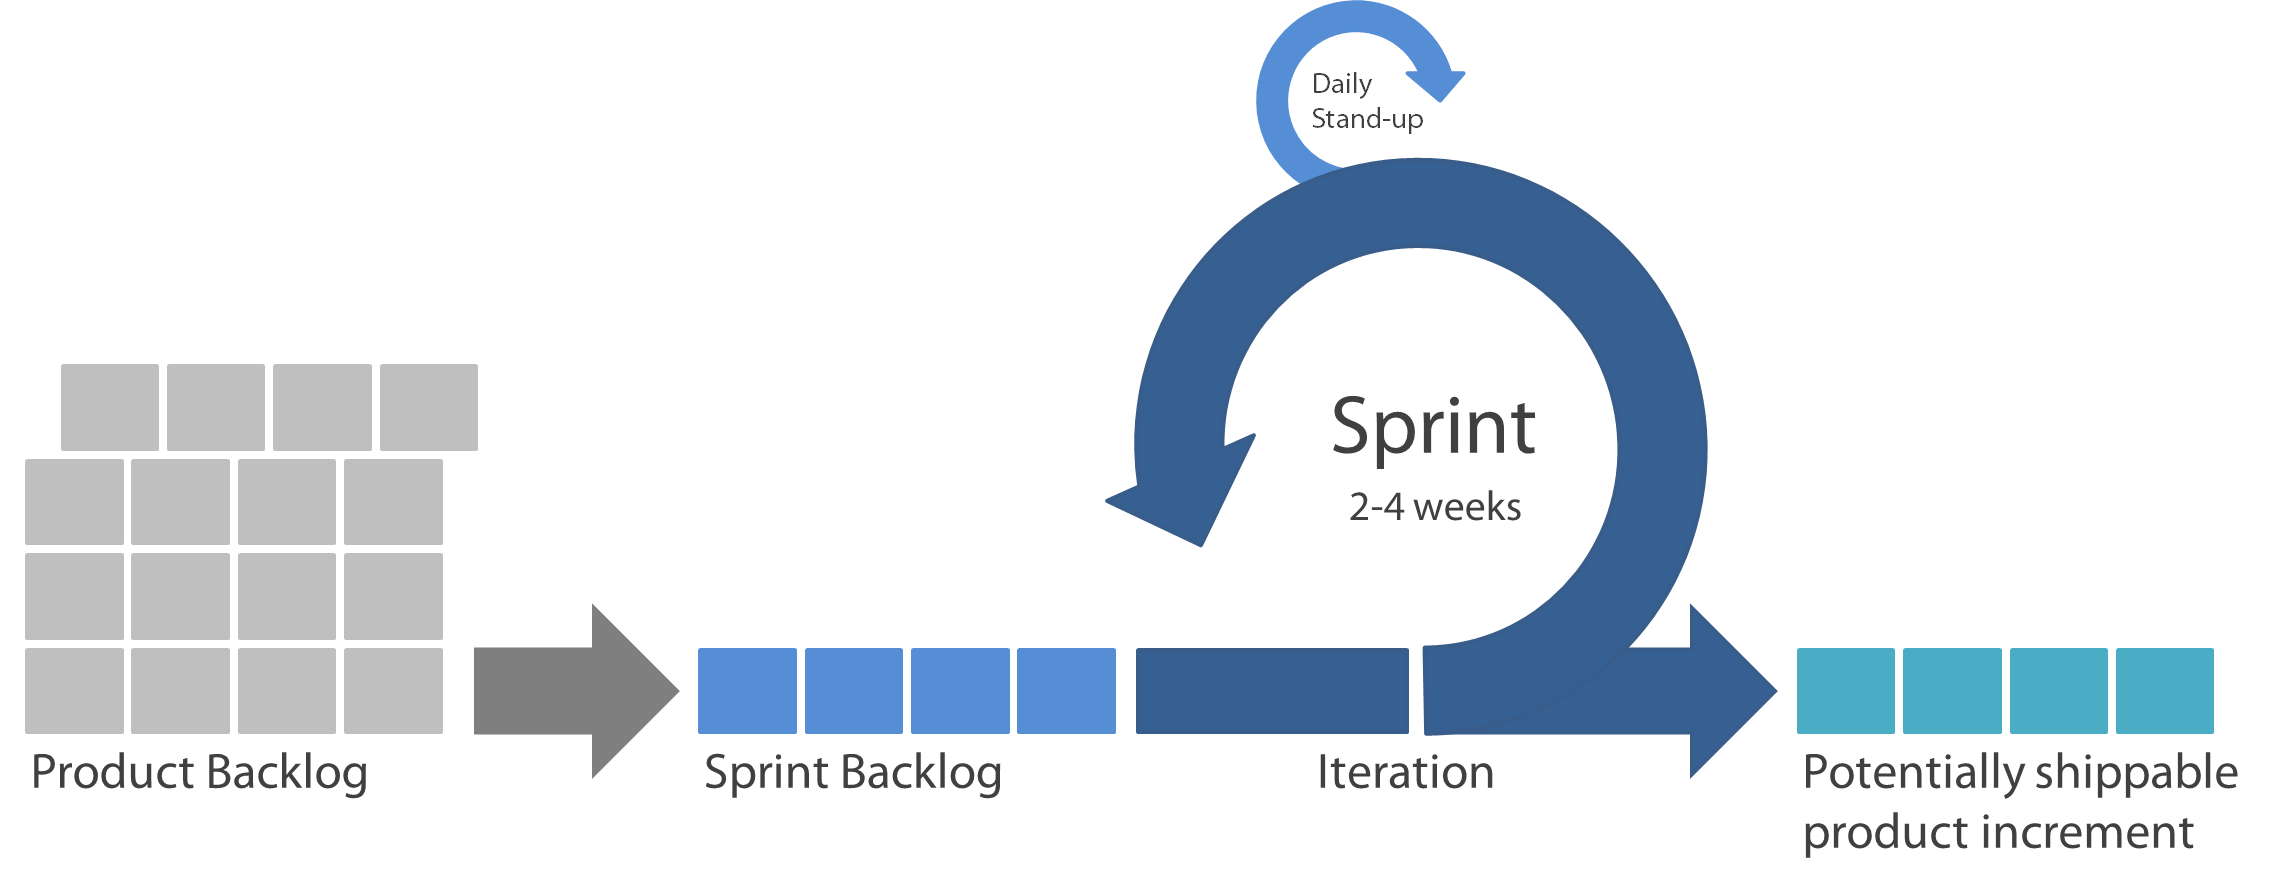
\includegraphics[width=0.9\textwidth]{scrum}
\caption{Ablauf eines Scrum-Sprints}
Quelle: \cite[][]{scrumbild}
\end{center}
\end{figure}
\vspace{-1cm}

\subsubsection{Scrum-Artefakte}
Während des Scrum-Prozesses werden einige Werkzeuge bzw. Artefakte genutzt. Zum einen werden die für das im Rahmen des Projekts zu enwickelnde System notwendigen Anforderungen im Product Backlog definiert. Dieses wird vom Product Owner erstellt und kontinuierlich geflegt. Es ist niemals vollständig, da sich die Anforderungen laufend ändern und dementsprechend muss das Dokument ebenfalls stetig  angepasst werden. Zum anderen wird aus diesem Product Backlog ein Sprint Backlog definiert, welches die für den aktuellen Sprint umzusetzenden Aktivitäten enthält. Diese werden durch das Team ausgewählt, in Aufgaben mit einer Implementierungsdauer von 4-16 Stunden aufgeteilt und in eine Reihenfolge gebracht. Es stellt somit ein Echtzeitabbild der in diesem Sprint durchzuführenden Aufgaben dar. Außerdem werden am Ende eines Sprints potenziell auslieferbare Inkremente erzeugt. Damit diese Funktionalitäten kurzfristig implementierbar sind, müssen sie aus qualitativ hochwertigem und gründlich getestetem Code bestehen. Zusätzlich müssen die in diesem Inkrement implementierten Funktionalitäten in irgendeiner Form für den Anwender dokumentiert sein.\footcite[Vgl.][Seite 10-15]{schwabo} 